%I need to make sure that I define subproblems clearly here to mean SRSs with rewrite rules. That's going to be a bit later.

\chapter{Hardness of Application of Rewrite Rules} \label{sec:hardnessrewriterules}
Now we have explained the background for Rewrite Systems, as well as the motivation for them, we now repeat the algebraic hardness measure computation done in section~\ref{sec:subhrdnspred} with a couple of changes: First, we do computations with a slightly modified Collatz SRS, and second, we only compute record sequences from our previous algebraic analysis. In this section, we first introduce a modified version of the SRS, then we define measures, talk about the computation, then present our results.

\subsection{Modified Base 8 Rewrite System} \label{subsec:base8rewrite}
Recall the Collatz SRS, and the $D$ rules: the rules that handle the even and odd numbers:
\begin{align*}
    D_1: ad &\rightarrow d &\text{$0\Mod{2}$}\\
    D_2: bd &\rightarrow gd &\text{$1\Mod{2}$}\\
\end{align*}
$D_1$ handles $0 \Mod{2}$ (even numbers) by effectively dividing by 2, while $D_2$ handles $1 \Mod{2}$ (odd numbers)  by effectively computing $3x+1/2$. Also note that all input strings for these rules are just one bit, since the placeholder $d$ is not a digit. However, we can expand this input to be 3 bits and come up with 8 corresponding SRRs:
\begin{align*}
    aaad &\rightarrow aad &\text{$0\Mod{8}$}\\
    aabd &\rightarrow ebad &\text{$1\Mod{8}$}\\
    abad &\rightarrow abd &\text{$2\Mod{8}$}\\
    abbd &\rightarrow fbbd &\text{$3\Mod{8}$}\\
    baad &\rightarrow bad &\text{$4\Mod{8}$}\\
    babd &\rightarrow gaad &\text{$5\Mod{8}$}\\
    bbad &\rightarrow bbd &\text{$6\Mod{8}$}\\
    bbbd &\rightarrow gbbd &\text{$7\Mod{8}$}
\end{align*}
These rules all correspond to a node in graph $G_8$. All of the odd rules, like rule $D_2$ in the original system, are just a combination of several rules, which ensure that the output string is not longer, and it reduces a couple of steps by moving the ternary term toward the front. However, all of the even number node rules are just the same exact rule $D_1$ in the original system. Hence, we can simplify this system and come up with the following SRRs:
\begin{align*}
    D_{8_1}: ad &\rightarrow d &\text{$0\Mod{2}$}\\
    D_{8_2}: aabd &\rightarrow ebd &\text{$1\Mod{8}$}\\
    D_{8_3}: abbd &\rightarrow fbbd &\text{$3\Mod{8}$}\\
    D_{8_4}: babd &\rightarrow gd &\text{$5\Mod{8}$}\\
    D_{8_5}: bbbd &\rightarrow gbbd &\text{$7\Mod{8}$}
\end{align*}
Because these rules were constructed using only SRRs in the Collatz SRS that we know to be correct, we know these new $D$ rules, plus the $A$, $B$, and $C$ rules, are equal to the original Collatz SRS. However, they do add an extra dimension not present before. We can remove one of the rules, for example rule $D_{8_2}$, and get this:
\begin{align*}
    D_{8_1}: ad &\rightarrow d &\text{$0\Mod{2}$}\\
    D_{8_3}: abbd &\rightarrow fbbd &\text{$3\Mod{8}$}\\
    D_{8_4}: babd &\rightarrow gd &\text{$5\Mod{8}$}\\
    D_{8_5}: bbbd &\rightarrow gbbd &\text{$7\Mod{8}$}
\end{align*}
These SRRs are equivalent to the Collatz Variant $Col(N,\{1\},8)$ defined in Algorithm~\ref{alg:SP}, since if we hit $1 \Mod{8}$, the input to the SRS terminates. Therefore, we can design an SRS for each of the subproblems 1, 5, and $7 \Mod{8}$ we investigated earlier, and determine the number of steps the systems take.

\subsection{Defining Measures} \label{subsec:rewritemeasuredefs}
Instead of defining hardness by number of odd numbers, for the SRS, we define hardness based off of the total steps applied. This is because an odd number adds a significant more number of rewrite steps... $\Theta(m)$ for the odd number, compared to just 1 for an even number. Define the following numbers, given some input number $x$:
\begin{itemize}
    \item $f_r(x)$: The total number of rewrite steps in the sequence for $x$ before it converges to 1.
    \item $A$: The base avoidance set. $A \subseteq \{1, 5, 7\}$ and $A \ne \varnothing$.
    \item Record Sequence for $A \Mod{b}$: Same exact definition in the algebraic sequence. We only run rewrite systems for the record sequences we computed with the algebraic Collatz method, as running computation for strictly the rewrite system would take an extremely long time.
    \item $R(x, A, b):$ The number of rewrite steps that the record sequence for number $x$ avoids $A \Mod{b}$. 
\end{itemize}
We define only one hardness measure: $H_{SRS}$, where $H_{SRS} = \frac{R(x, A, b)}{\log_2{x}}$. This effectively computes the hardness of the SRRs that corresponds to avoiding $A \Mod{b}$.

\subsection{Computation} \label{subsec:rewritecomp}
The program I wrote simulates the Collatz SRS in Java. It takes two different keys of input: some positive integers (either one number, or a batch of numbers, one per line), and a string file which has one SRR per line in the format ``input output'', which is equivalent to the rule $input \rightarrow output$. The \# character is a comment, meaning if the first character of a rewrite rule is \#, we ignore that line. This is a convenience to comment out a rule to create SRRs that correspond to Collatz subproblems. \par
The program converts an input number into a binary rewrite string with characters $a$, $b$, $c$, and $d$. The rewrite term is stored in a ``sliding'' array, because in Aaronson's SRS, a number can only add string length from the $c$ rules. When we apply rule $D_{8_1}$, the $a$ term gets replaced with a $d$ term, and a pointer denoting the end of the string gets moved to the new $d$ symbol. If we run out of space in the array, we double the size of it, and discard any trailing $d$ terms. \par
As discussed in section~\ref{sec:CollatzSRS}, we don't apply SRRs in arbitrary order. Given a rewrite string completely in binary, we check to see if any $D$ rule can be applied. If not, the program terminates. If we do find a $D$ rule, then apply it, and check if a ternary character is generated by it. If so, we apply the $A$ and $B$ rules to move the ternary character index-by-index until we can apply a $C$ rule, which removes the ternary character.
Since omitting a SRR corresponds exactly to a certain subproblem $Col(N,A,b)$ for some base avoidance set $A$, we need to take the first number from record sequences computed algebraically that \textit{isn't} $Col(N,A,b)$, and run the SRS until it terminates. \par
The output is, for one number, the terms that result from the application of the SRRs until it terminates, as well as which number the intermediate terms correspond to. For a batch of numbers, each individual number is output in a separate file, and there is an overall file that outputs the input number, the final number, and the number of rewrite steps.

\subsection{Single SRR removal analysis} \label{subsec:rewritehardness}
Figure~\ref{fig:rvslog} shows the anaylsis of hardness for the modified SRS with removal on one of three different rules. Note that the hardness tends to grow for all three cases, as opposed to the analysis for $H(x,A)$ for each of these three cases, which tend to stay flat. This shows, that as the number of bits increases, the number of steps for the rewrite system tend to increase logarithmically. The best explanation for why this is the case is because for each odd rule, we add $\Theta(\log{n})$ steps, so as discussed in the algebraic case, hardness is determined by odd numbers.
\begin{figure}
    \centering
    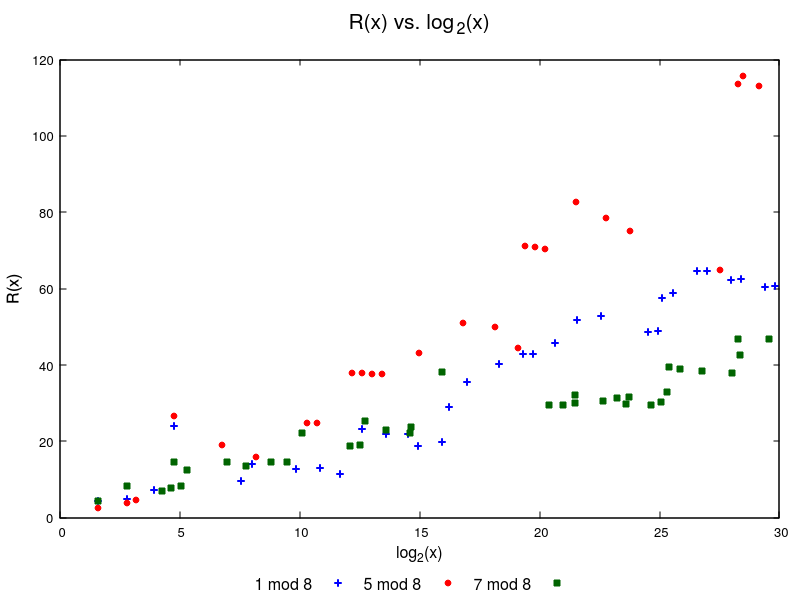
\includegraphics[scale=0.75]{ModAvoidanceAnalysisPics/R_vs_log.png}
    \caption{This graph visualizes how the $R$ values for $1 \Mod{8}$, $5 \Mod{8}$, and $7 \Mod{8}$ compare to each other. The log of the record holding numbers, or number of bits needed, is the x-axis, and the hardness measure $R$ as defined in section~\ref{subsec:rewritemeasuredefs} is the y-axis.}
    \label{fig:rvslog}
\end{figure}
However, it is clear that all three cases don't have the same slope of increase. $7 \Mod{8}$ has the most gradual growth of all three cases, followed by $1 \Mod{8}$ and $5 \Mod{8}$, which has not only the most growth, but the highest standard deviation of all three cases. These can be explained by the following observations:
\begin{itemize}
    \item Avoiding $7 \Mod{8}$ eliminates the growth of the $6 \rightarrow 7 \rightarrow 6$ cycle, meaning the numbers tend to get smaller and need less bits to encode as a rewrite string.
    \item Avoiding $5 \Mod{8}$ eliminates the decay of the 0 self-cycle, meaning numbers tend to grow more often than not, so the numbers here are larger.
    \item Avoiding $1 \Mod{8}$ is in between the other two cases, since both the 0 self-cycle of decay and the $6 \rightarrow 7 \rightarrow 6$ of growth can occur.
\end{itemize}
%This is all proof for showing how these rules correspond to the base 4 graph. I feel like this is unncessary for now, but I'll keep it in mind.
%We can actually expand our input strings to have two bits instead of 1, and with substitutions of certain rules, we can replace these two rules with 4 rules that results in an equivalent system. We also add a leading $x$ character, which means $x$ can be either $a$ or $b$.\footnote{$x$ could be any other character in the rewrite system except $d$, but none of these cases are interesting. If $x = c$, this system is nearly terminating, as this string corresponds to a number less than 8, which we know converges to 1. If $x$ is a ternary $e$, $f$, or $g$ character, then the $A$ and $B$ rules ensure we move the ternary character further left, so $x$ would turn into $a$ or $b$ as a result.} Here are the rules:
%\begin{align*}
%    D_1: xaad &\rightarrow xad &\text{$0\Mod{4}$}\\
%    D_2: xabd &\rightarrow xfad &\text{$1\Mod{4}$}\\
%    D_3: xbad &\rightarrow xbd &\text{$2\Mod{4}$}\\
%    D_4: xbbd &\rightarrow xgbd &\text{$3\Mod{4}$}
%\end{align*}
%These rules handle numbers based off of their last two bits, like the base 4 graph concerns the last 2 bits of numbers. Note that $D_1$ and $D_3$ in this new system are actually redundant rules. They could be replaced by the original $ad \rightarrow d$ rule and the system would function the same, but this example is just used to clearly show how the rewrite system ties to the graph. We do keep the odd rules in mind, as they will be important in simplifying the rewrite system down the road, particularly rule $D_4$. \par
%We now show how these rules correspond to the mod 4 graph. First, look at rules $D_1$ and $D_3$, the even rules. Both divide by 2, so an $a$ disappears. We look at the value for $x$ to determine what the new mod 4 value will be. For $D_1$, if $x$ is $a$, we end the string with $aad$, or $0 (\Mod{4})$, and we've hit the self loop of the graph, repeating rule $D_1$ for the next step. Else, if $x$ is $b$, we now have the string ending with $bad$, or $0 (\Mod{4})$, and apply rule $D_3$, also like in the graph. For $D_3$, in both cases, we end up with an odd number, because we end with a $b$, denoting a 1 bit, so if $x$ is $a$, we have $abd$, or $1 (\Mod{4})$, and if $x$ is $b$, we have $bbd$, or $3 (\Mod{4})$.\par
%The odd rules are trickier to explain, because the initial $bd \rightarrow gd$ rule, as discussed, actually computes $\frac{3x+1}{2}$. Hence, applying either of these rules actually results in a corresponding jump of two nodes. Since we've established the even nodes as having the correct transitions in the graphs, we can identify which node we go to given the transitions after applying rules $D_2$ and $D_4$. For $D_2$, if $x$ is $a$, we apply rule $A_2$, $af \rightarrow eb$, meaning our string ends with $bad$, so our next $D$ rule will be $D_3$. If $x$ is $b$, we apply $B_2$, $bf \rightarrow ga$, so our string ends with $aad$, and we apply $D_1$. This suggests that $D_2$ must transition to $0 (\Mod{4})$ because $0 (\Mod{4})$ can transition to rules $D_1$ or $D_3$, but not $2 (\Mod{4})$. This agrees with our graph. \par
%For $D_4$, if $x$ is $a$, then we apply rule $A_3$: $ag \rightarrow fa$. Our string ends with $abd$, so we're at $1 (\Mod{4})$, and apply rule $D_2$. Else, if $x$ is $b$, we apply rule $B_3$: $bg \rightarrow gb$, making our string end with $bbd$, and we apply rule $D_4$ once again. These paths correspond to coming from the $2 (\Mod{4})$ node, meaning $3 (\Mod{4})$ transitions to $2 (\Mod{4})$. Hence, this also agrees with the graph, and all of the $D$ rules in the new system agree with the graph. \par
%\subsection{Base 8 graph and rewrite tie together}
%Here are rewrite rules that correspond to this graph:
%These are now above.
%We omitted the $x$ this time, as we won't prove that they correspond to the graph. The approach is similar to what we had for base 4. Once again, the even rules are redundant, but the odd rules will be helpful in constructing a more efficient revised system. \par